\documentclass{article}

  % packages
    % basic stuff for rendering math
    \usepackage[letterpaper, top=1in, bottom=1in, left=1in, right=1in]{geometry}
    \usepackage[utf8]{inputenc}
    \usepackage[english]{babel}
    \usepackage{amsmath} 
    \usepackage{amssymb}
    \usepackage{bbm}

    % extra math symbols and utilities
    \usepackage{mathtools}        % for extra stuff like \coloneqq
    \usepackage{mathrsfs}         % for extra stuff like \mathsrc{}
    \usepackage{centernot}        % for the centernot arrow 
    \usepackage{bm}               % for better boldsymbol/mathbf 
    \usepackage{enumitem}         % better control over enumerate, itemize
    \usepackage{hyperref}         % for hypertext linking
    \usepackage{xr-hyper}
    \usepackage{fancyvrb}          % for better verbatim environments
    \usepackage{newverbs}         % for texttt{}
    \usepackage{xcolor}           % for colored text 
    \usepackage{listings}         % to include code
    \usepackage{lstautogobble}    % helper package for code
    \usepackage{parcolumns}       % for side by side columns for two column code
    

    % page layout
    \usepackage{fancyhdr}         % for headers and footers 
    \usepackage{lastpage}         % to include last page number in footer 
    \usepackage{parskip}          % for no indentation and space between paragraphs    
    \usepackage[T1]{fontenc}      % to include \textbackslash
    \usepackage{footnote}
    \usepackage{etoolbox}

    % for custom environments
    \usepackage{tcolorbox}        % for better colored boxes in custom environments
    \tcbuselibrary{breakable}     % to allow tcolorboxes to break across pages

    % figures
    \usepackage{pgfplots}
    \pgfplotsset{compat=1.18}
    \usepackage{float}            % for [H] figure placement
    \usepackage{tikz}
    \usepackage{tikz-cd}
    \usepackage{circuitikz}
    \usetikzlibrary{arrows, shapes.geometric}
    \usetikzlibrary{positioning}
    \usetikzlibrary{calc}
    \usepackage{graphicx}
    \usepackage{algorithmic}
    \usepackage{caption} 
    \usepackage{subcaption}
    \captionsetup{font=small}

    % for tabular stuff 
    \usepackage{dcolumn}

    \usepackage[nottoc]{tocbibind}
    \pdfsuppresswarningpagegroup=1
    \hfuzz=5.002pt                % ignore overfull hbox badness warnings below this limit

  % New and replaced operators
    \DeclareMathOperator{\Tr}{Tr}
    \DeclareMathOperator{\Sym}{Sym}
    \DeclareMathOperator{\Span}{span}
    \DeclareMathOperator{\std}{std}
    \DeclareMathOperator{\Cov}{Cov}
    \DeclareMathOperator{\Var}{Var}
    \DeclareMathOperator{\Corr}{Corr}
    \DeclareMathOperator{\pos}{pos}
    \DeclareMathOperator*{\argmin}{\arg\!\min}
    \DeclareMathOperator*{\argmax}{\arg\!\max}
    \newcommand{\ket}[1]{\ensuremath{\left|#1\right\rangle}}
    \newcommand{\bra}[1]{\ensuremath{\left\langle#1\right|}}
    \newcommand{\braket}[2]{\langle #1 | #2 \rangle}
    \newcommand{\qed}{\hfill$\blacksquare$}     % I like QED squares to be black

  % Custom Environments
    \newtcolorbox[auto counter, number within=section]{question}[1][]
    {
      colframe = orange!25,
      colback  = orange!10,
      coltitle = orange!20!black,  
      breakable, 
      title = \textbf{Question \thetcbcounter ~(#1)}
    }

    \newtcolorbox[auto counter, number within=section]{exercise}[1][]
    {
      colframe = teal!25,
      colback  = teal!10,
      coltitle = teal!20!black,  
      breakable, 
      title = \textbf{Exercise \thetcbcounter ~(#1)}
    }
    \newtcolorbox[auto counter, number within=section]{solution}[1][]
    {
      colframe = violet!25,
      colback  = violet!10,
      coltitle = violet!20!black,  
      breakable, 
      title = \textbf{Solution \thetcbcounter}
    }
    \newtcolorbox[auto counter, number within=section]{lemma}[1][]
    {
      colframe = red!25,
      colback  = red!10,
      coltitle = red!20!black,  
      breakable, 
      title = \textbf{Lemma \thetcbcounter ~(#1)}
    }
    \newtcolorbox[auto counter, number within=section]{theorem}[1][]
    {
      colframe = red!25,
      colback  = red!10,
      coltitle = red!20!black,  
      breakable, 
      title = \textbf{Theorem \thetcbcounter ~(#1)}
    } 
    \newtcolorbox[auto counter, number within=section]{proposition}[1][]
    {
      colframe = red!25,
      colback  = red!10,
      coltitle = red!20!black,  
      breakable, 
      title = \textbf{Proposition \thetcbcounter ~(#1)}
    } 
    \newtcolorbox[auto counter, number within=section]{corollary}[1][]
    {
      colframe = red!25,
      colback  = red!10,
      coltitle = red!20!black,  
      breakable, 
      title = \textbf{Corollary \thetcbcounter ~(#1)}
    } 
    \newtcolorbox[auto counter, number within=section]{proof}[1][]
    {
      colframe = orange!25,
      colback  = orange!10,
      coltitle = orange!20!black,  
      breakable, 
      title = \textbf{Proof. }
    } 
    \newtcolorbox[auto counter, number within=section]{definition}[1][]
    {
      colframe = yellow!25,
      colback  = yellow!10,
      coltitle = yellow!20!black,  
      breakable, 
      title = \textbf{Definition \thetcbcounter ~(#1)}
    } 
    \newtcolorbox[auto counter, number within=section]{example}[1][]
    {
      colframe = blue!25,
      colback  = blue!10,
      coltitle = blue!20!black,  
      breakable, 
      title = \textbf{Example \thetcbcounter ~(#1)}
    } 
    \newtcolorbox[auto counter, number within=section]{code}[1][]
    {
      colframe = green!25,
      colback  = green!10,
      coltitle = green!20!black,  
      breakable, 
      title = \textbf{Code \thetcbcounter ~(#1)}
    } 
    \newtcolorbox[auto counter, number within=section]{algo}[1][]
    {
      colframe = green!25,
      colback  = green!10,
      coltitle = green!20!black,  
      breakable, 
      title = \textbf{Algorithm \thetcbcounter ~(#1)}
    } 

    \definecolor{dkgreen}{rgb}{0,0.6,0}
    \definecolor{gray}{rgb}{0.5,0.5,0.5}
    \definecolor{mauve}{rgb}{0.58,0,0.82}
    \definecolor{darkblue}{rgb}{0,0,139}
    \definecolor{lightgray}{gray}{0.93}
    \renewcommand{\algorithmiccomment}[1]{\hfill$\triangleright$\textcolor{blue}{#1}}

    % default options for listings (for code)
    \lstset{
      autogobble,
      frame=ltbr,
      language=Python,
      aboveskip=3mm,
      belowskip=3mm,
      showstringspaces=false,
      columns=fullflexible,
      keepspaces=true,
      basicstyle={\small\ttfamily},
      numbers=left,
      firstnumber=1,                        % start line number at 1
      numberstyle=\tiny\color{gray},
      keywordstyle=\color{blue},
      commentstyle=\color{dkgreen},
      stringstyle=\color{mauve},
      backgroundcolor=\color{lightgray}, 
      breaklines=true,                      % break lines
      breakatwhitespace=true,
      tabsize=3, 
      xleftmargin=2em, 
      framexleftmargin=1.5em, 
      stepnumber=1
    }

  % Page style
    \pagestyle{fancy}
    \fancyhead[L]{Trees}
    \fancyhead[C]{Muchang Bahng}
    \fancyhead[R]{Spring 2025} 
    \fancyfoot[C]{\thepage / \pageref{LastPage}}
    \renewcommand{\footrulewidth}{0.4pt}          % the footer line should be 0.4pt wide
    \renewcommand{\thispagestyle}[1]{}  % needed to include headers in title page

  % external documents 
  %  \externaldocument[place-]{../Machine_Learning/paper}[../Machine_Learning/paper.pdf] 

\begin{document}

\title{Trees}
\author{Muchang Bahng}
\date{Spring 2025}

\maketitle
\tableofcontents
\pagebreak 

This covers computability theory, complexity theory, and automata theory. 
Alphabet. Boolean logic


\section{Decision Trees} 

  In here, we define the decision tree model. It is most natural for classification, but there are variants of it for regression.   

  Many discriminative models can be written in a clean formula (e.g. $y = w^T x + \epsilon$ for linear regression, and even $y = \prod_i (\sigma_i \circ A_i) (x)$ for MLPs). However, we cannot find such a parameteric form for a tree, which is why they are nonparametric models. In full generality, all we can say is that they have a general tree structure, and there are many variants. 

\subsection{Classification Trees}

  \begin{definition}[Classification Trees] 
    A \textbf{decision/classification tree} is a nonparameteric discriminative model $f$ that creates some sort of tree representing a set of decisions on an input $x$ to predict a label $y$. 

    \begin{figure}[H]
      \centering 
      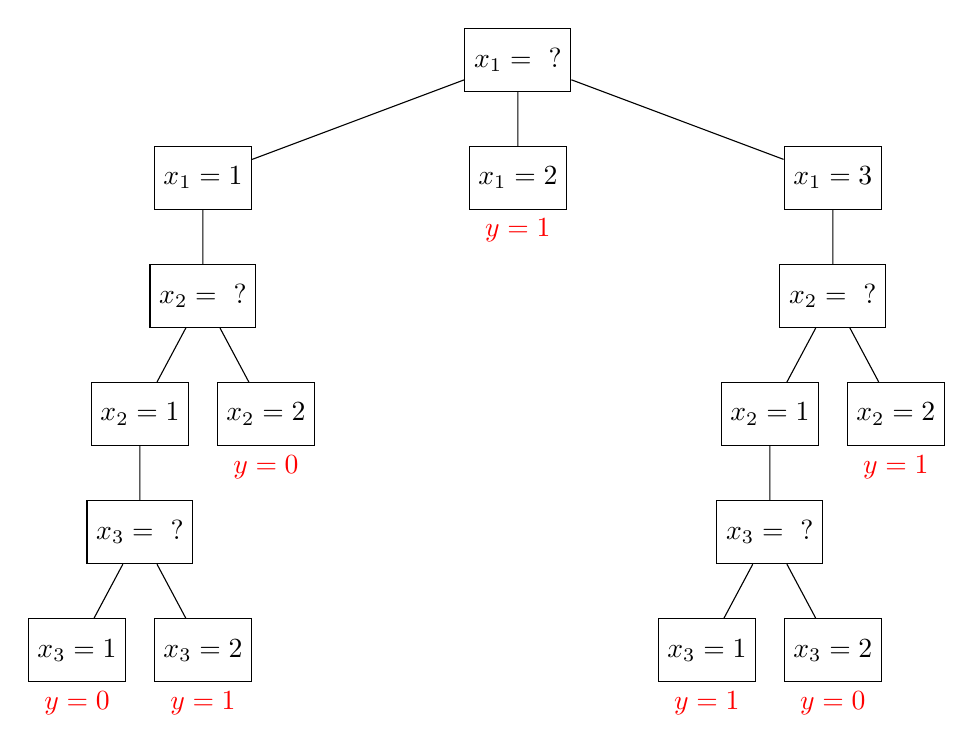
\begin{tikzpicture}[
        level 1/.style={sibling distance=40mm},  % Increased from 48mm
        level 2/.style={sibling distance=20mm},  % Increased from 16mm
        level 3/.style={sibling distance=16mm},  % Increased from 8mm
        box/.style={draw, rectangle, minimum width=12mm, minimum height=8mm},
        edge from parent/.style={draw, -}  % Added for cleaner look
      ]
        \node[box] {$x_1=\text{ ?}$}
          % Level 1
          child {
            node[box] {$x_1=1$}
            child {
              node[box] {$x_2=\text{ ?}$}
              child {
                node[box] {$x_2=1$}
                child {
                  node[box] {$x_3=\text{ ?}$}
                  child {
                    node[box] {$x_3=1$}
                    node[below=4mm] {\textcolor{red}{$y=0$}}
                  }
                  child {
                    node[box] {$x_3=2$}
                    node[below=4mm] {\textcolor{red}{$y=1$}}
                  }
                }
              }
              child {
                node[box] {$x_2=2$}
                node[below=4mm] {\textcolor{red}{$y=0$}}
              }
            }
          }
          % Middle branch
          child {
            node[box] {$x_1=2$}
            node[below=4mm] {\textcolor{red}{$y=1$}}
          }
          % Right branch
          child {
            node[box] {$x_1=3$}
            child {
              node[box] {$x_2=\text{ ?}$}
              child {
                node[box] {$x_2=1$}
                child {
                  node[box] {$x_3=\text{ ?}$}
                  child {
                    node[box] {$x_3=1$}
                    node[below=4mm] {\textcolor{red}{$y=1$}}
                  }
                  child {
                    node[box] {$x_3=2$}
                    node[below=4mm] {\textcolor{red}{$y=0$}}
                  }
                }
              }
              child {
                node[box] {$x_2=2$}
                node[below=4mm] {\textcolor{red}{$y=1$}}
              }
            }
          };
      \end{tikzpicture}
      \caption{An example of a decision tree that splits at $x_1$ first, then $x_2$, and finally $x_3$. Note that you can still split on $x_2$ if $x_1 = 1$ and $x_3$ if $x_1 = 3$. } 
      \label{fig:decision_tree}
    \end{figure}
  \end{definition}

  The decision tree tries to take advantage of some nontrivial covariance between $X$ and $Y$ by constructing nested partitions of the dataset $\mathcal{D}$, and within a partition, it predicts the label that comprises the majority. 

  For now, let us assume that $\mathcal{X}$ is a Cartesian product of discrete sets, and we will extend them to continuous values later. Let us look at an example to gain some intuition. 

  \begin{example}[Restaurant Dataset]
    Consider the following dataset. 

    \begin{table}[H]
      \centering
      {\footnotesize 
      \begin{tabular}{|c|c|c|c|c|c|c|c|c|c|c|}
        \hline
        & OthOptions & Weekend & WaitArea & Plans & Price & Precip & Restaur & Wait & Crowded & Stay? \\
        \hline
        $x_1$ & \textcolor{blue}{Yes} & \textcolor{blue}{No} & \textcolor{blue}{No} & \textcolor{blue}{Yes} & \$\$\$ & \textcolor{blue}{No} & \textcolor{blue}{Mateo} & 0-5 & \textcolor{blue}{some} & Yes \\
        \hline
        $x_2$ & \textcolor{green!50!black}{Yes} & \textcolor{green!50!black}{No} & \textcolor{green!50!black}{No} & \textcolor{green!50!black}{Yes} & \$ & \textcolor{green!50!black}{No} & \textcolor{green!50!black}{Juju} & 16-30 & \textcolor{green!50!black}{full} & No \\
        \hline
        $x_3$ & \textcolor{blue}{No} & \textcolor{blue}{No} & \textcolor{blue}{Yes} & \textcolor{blue}{No} & \$ & \textcolor{blue}{No} & \textcolor{blue}{Pizza} & 0-5 & \textcolor{blue}{some} & Yes \\
        \hline
        $x_4$ & \textcolor{blue}{Yes} & \textcolor{blue}{Yes} & \textcolor{blue}{No} & \textcolor{blue}{Yes} & \$ & \textcolor{blue}{No} & \textcolor{blue}{Juju} & 6-15 & \textcolor{blue}{full} & Yes \\
        \hline
        $x_5$ & \textcolor{green!50!black}{Yes} & \textcolor{green!50!black}{Yes} & \textcolor{green!50!black}{No} & \textcolor{green!50!black}{No} & \$\$\$ & \textcolor{green!50!black}{No} & \textcolor{green!50!black}{Mateo} & 30+ & \textcolor{green!50!black}{full} & No \\
        \hline
        $x_6$ & \textcolor{blue}{No} & \textcolor{blue}{No} & \textcolor{blue}{Yes} & \textcolor{blue}{Yes} & \$\$ & \textcolor{blue}{Yes} & \textcolor{blue}{BlueCorn} & 0-5 & \textcolor{blue}{some} & Yes \\
        \hline
        $x_7$ & \textcolor{green!50!black}{No} & \textcolor{green!50!black}{No} & \textcolor{green!50!black}{Yes} & \textcolor{green!50!black}{No} & \$ & \textcolor{green!50!black}{Yes} & \textcolor{green!50!black}{Pizza} & 0-5 & \textcolor{green!50!black}{none} & No \\
        \hline
        $x_8$ & \textcolor{blue}{No} & \textcolor{blue}{No} & \textcolor{blue}{No} & \textcolor{blue}{Yes} & \$\$ & \textcolor{blue}{Yes} & \textcolor{blue}{Juju} & 0-5 & \textcolor{blue}{some} & Yes \\
        \hline
        $x_9$ & \textcolor{green!50!black}{No} & \textcolor{green!50!black}{Yes} & \textcolor{green!50!black}{Yes} & \textcolor{green!50!black}{No} & \$ & \textcolor{green!50!black}{Yes} & \textcolor{green!50!black}{Pizza} & 30+ & \textcolor{green!50!black}{full} & No \\
        \hline
        $x_{10}$ & \textcolor{green!50!black}{Yes} & \textcolor{green!50!black}{Yes} & \textcolor{green!50!black}{Yes} & \textcolor{green!50!black}{Yes} & \$\$\$ & \textcolor{green!50!black}{No} & \textcolor{green!50!black}{BlueCorn} & 6-15 & \textcolor{green!50!black}{full} & No \\
        \hline
        $x_{11}$ & \textcolor{green!50!black}{No} & \textcolor{green!50!black}{No} & \textcolor{green!50!black}{No} & \textcolor{green!50!black}{No} & \$ & \textcolor{green!50!black}{No} & \textcolor{green!50!black}{Juju} & 0-5 & \textcolor{green!50!black}{none} & No \\
        \hline
        $x_{12}$ & \textcolor{blue}{Yes} & \textcolor{blue}{Yes} & \textcolor{blue}{Yes} & \textcolor{blue}{Yes} & \$ & \textcolor{blue}{No} & \textcolor{blue}{Pizza} & 16-30 & \textcolor{blue}{full} & Yes \\
        \hline
      \end{tabular}
      }
      \caption{Dataset of whether to go to a restaurant for a date depending on certain factors. }
      \label{tab:restaurant}
    \end{table}

    Let us denote $\mathcal{D}$ as the dataset, and say that $F_1, \ldots, F_d$ were the features. This is a binary classification problem, and we can count that there are $6$ positives and $6$ negative labels. 
  \end{example}

  The simplest decision tree is the trivial tree, with one node that predicts the majority of the dataset. In this case, the data is evenly split, so without loss of generality we will choose $h_0 (\mathbf{x}) = 1$. We want to quantify how good our model is, and so like always we use a loss function. 

  Just like how a linear model is completely defined by its parameter $\boldsymbol{\theta}$, a decision tree is completely defined by the sequences of labels that it splits on. Therefore, training this is equivalent to defining the sequence, but we can't define this sequence unless we can compare how good a given decision tree is, i.e. unless we have defined a proper loss function. Depending on the training, we can use a greedy algorithm or not, and we have the flexibility to choose whether or not we can split on the same feature multiple times. 

  \begin{definition}[Misclassification Error]
    We will simply use the misclassification loss function. 
    \begin{equation}
      L(h; \mathcal{D}) = \frac{1}{N} \sum_{i=1}^N 1_{\{y^{(i)} \neq h(x^{(i)})\}} = 1 - \text{accuracy}
    \end{equation}
    Minimizing this maximizes the accuracy, so this is a reasonable one to choose. How do we train this? Unlike regression, this loss is not continuous, so the gradient is $0$, and furthermore the model isn't even parametric, so there are no gradients to derive! 
  \end{definition}

  Fortunately, the nature of the decision tree only requires us to look through the explanatory variables $x_1, \ldots, x_n$ and decide which one to split. 

  Let us take a decision tree $h$ and model the accuracy of it as a random variable: $1_{\{Y = h_0 (X)\}} \sim \mathrm{Bernoulli}(p)$, where $p$ is the accuracy. A higher accuracy of $h$ corresponds to a lower entropy, and so the entropy of the random variable is also a relevant indicator. 
  \[H(1_{\{Y = h_0 (X)\}}) = p \log{p} + (1 - p) \log(1 - p)\]
  Therefore, when we are building a tree, we want to choose the feature $x_i$ to split based on how much it lowers the entropy of the decision tree. 

  To set this up, let us take our dataset $\mathcal{D}$ and set $X_i$ as the random variable representing the distribution (a multinomial) of the $x_i^{(j)}$'s, and $Y$ as the same for the $y^{(j)}$'s. This is our maximum likelihood approximation for the marginalized distribution of the joint measure $X \times Y = X_1 \times \ldots \times X_D \times Y$. 

  Given a single node, we are simply going to label every point to be whatever the majority class is in $\mathcal{D}$. Therefore, we start off with the entropy of our trivial tree $H(Y)$. Then, we want to see which one of the $X_d$ features to split on, and so we can compute the conditional entropy $H(Y, X_d)$ to get the information gain $I(Y; X_d) = H(Y) - H(Y \mid X_d)$ for all $d = 1, \ldots, D$. We want to find a feature $X_d$ that maximize this information gain, i.e. decreases the entropy as much as possible (a greedy algorithm), and we find the next best feature (with or without replacement), so that we have a decreasing sequence. 
  \[H(X) \geq H(X ; Y) \geq H(X ; Y, Z) \geq H(X ; Y, Z, W) \geq \ldots \geq 0\]

  \begin{example}[Crowded Restaurants]
    Continuing the example above, since there are $6$ labels of $0$ and $1$ each, we can model this $Y \sim \mathrm{Bernoulli}(0.5)$ random variable, with entropy 
    \begin{equation}
      H(Y) = \mathbb{E}[-\log_2 p(Y)] = \frac{1}{2} \big( -\log_2 \frac{1}{2} \big) + \frac{1}{2} \big( -\log_2 \frac{1}{2} \big) = 1
    \end{equation}

    Now what would happen if we had branched according to how crowded it was, $X_{\mathrm{crowded}}$. Then, our decision tree would split into 3 sections: 
    \begin{figure}[H]
      \centering 
      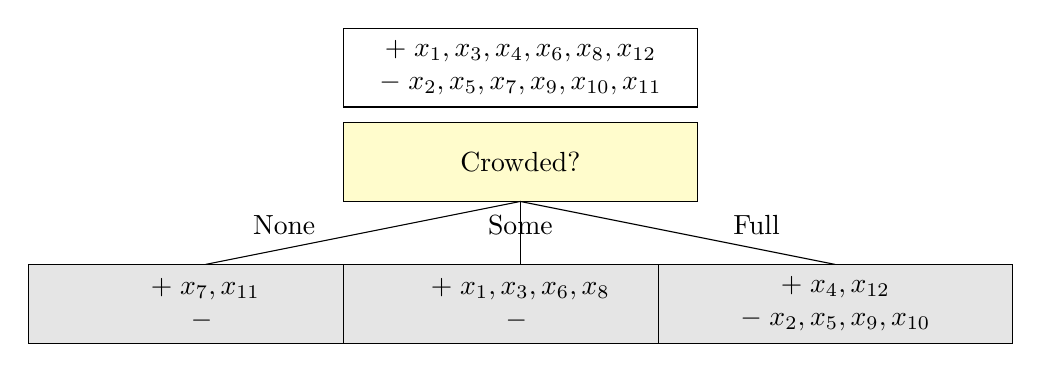
\begin{tikzpicture}[
        box/.style={draw, rectangle, minimum width=4.5cm, minimum height=1cm, align=center},
        yellowbox/.style={box, fill=yellow!20},
        graybox/.style={box, fill=gray!20},
        level 1/.style={sibling distance=6cm},
        level 2/.style={sibling distance=3cm},
        edge from parent/.style={draw, -}
      ]
        % Root node
        \node[box] {$+ \; x_1,x_3,x_4,x_6,x_8,x_{12}$ \\ $- \; x_2,x_5,x_7,x_9,x_{10},x_{11}$};
        \node[yellowbox] at (0,-1.2) {Crowded?};
        
        % Level 1 nodes and edges
        \node[graybox] at (-4,-3) {$+ \; x_7,x_{11}$ \\ $- \; $};
        \node[graybox] at (0,-3) {$+ \; x_1,x_3,x_6,x_8$ \\ $- \; $};
        \node[graybox] at (4,-3) {$+ \; x_4,x_{12}$ \\ $- \; x_2,x_5,x_9,x_{10}$};
        
        % Draw edges
        \draw (0,-1.7) -- (-4,-2.5);
        \draw (0,-1.7) -- (0,-2.5);
        \draw (0,-1.7) -- (4,-2.5);
        
        % Labels for edges
        \node at (-3,-2) {None};
        \node at (0,-2) {Some};
        \node at (3,-2) {Full};
      \end{tikzpicture}
      \caption{Visual of decision tree splitting according to how crowded it is. } 
      \label{fig:crowded_restaurants}
    \end{figure}
    
    In this case, we can define the multinomial distribution $X_{\mathrm{crowded}}$ representing the proportion of the data that is crowded in a specific level. That is, $X_{\mathrm{crowded}} \sim \mathrm{Multinomial}(\frac{2}{12}, \frac{4}{12}, \frac{6}{12} \big)$, with 
    \begin{equation}
      \mathbb{P}(X_{\mathrm{crowded}} = x) = \begin{cases} 2/12 & \text{ if } x = \text{ none} \\ 4/12 & \text{ if } x = \text{ some} \\ 6/12 & \text{ if } x = \text{ full} \end{cases}
    \end{equation}
    Therefore, we can now compute the conditional entropy of this new decision tree conditioned on how crowded the store is 
    \begin{align}
      H(Y \mid X_{\mathrm{crowded}}) & = \sum_x \mathbb{P}(X_{\mathrm{crowded}} = x) H(Y \mid X_{\mathrm{crowded}} = x) \\
      & = \frac{2}{12} H(\mathrm{Bern}(1)) + \frac{4}{12} H(\mathrm{Bern}(0)) + \frac{6}{12} H(\mathrm{Bern}(1/3)) = 0.459 \\
      I(Y; X_{\mathrm{crowded}}) & = 0.541
    \end{align}
    We would do this for all the features and greedily choose the feature that maximizes our information gain. 
  \end{example}

  \begin{example}[Ferrari F1 Race]
    The Ferrari F1 team hired you as a new analyst! You were given the following table of the past race history of the team. You were asked to use information gain to build a decision tree to predict race wins. First, you will need to figure out which feature to split first. 
    \begin{center}
      \begin{tabular}[c]{c|c|c||c}
      Rain & Good Strategy & Qualifying & Win Race \\ \hline
      1 & 0 & 0 & 0 \\
      1 & 0 & 0 & 0 \\
      1 & 0 & 1 & 0 \\
      0 & 0 & 1 & 1 \\
      0 & 0 & 0 & 0 \\
      0 & 1 & 1 & 1 \\
      1 & 0 & 1 & 0 \\
      0 & 1 & 0 & 1 \\
      0 & 0 & 1 & 1 \\
      0 & 0 & 1 & 1 \\
      \end{tabular}
    \end{center}

    Let $X \sim \mathrm{Bernoulli}(1/2)$ be the distribution of whether a car wins a race over the data. Then its entropy is 
    \begin{equation}
      H(X) = \mathbb{E}[-\log_2 p(x)] = \frac{1}{2} \big( -\log_2 \frac{1}{2} \big) + \frac{1}{2} \big( -\log_2 \frac{1}{2} \big) = 1
    \end{equation}

    Let $R \sim \mathrm{Bernoulli}(4/10), G \sim \mathrm{Bernoulli}(2/10), Q \sim \mathrm{Bernoulli}(6/10)$ be the distribution of the features rain, good strategy, and qualifying over the data, respectively. Then, the conditional entropy of $X$ conditioned on each of these random variables is 
    \begin{align*}
      H(X \mid R) & = \mathbb{P}(R = 1)\, H(X \mid R = 1) + \mathbb{P}(R = 0) \, H(X \mid R = 0) \\
      & = \frac{4}{10} \cdot - \big( 1 \cdot \log_2 1 + 0 \cdot \log_2 0 \big) + \frac{6}{10} \cdot - \big( \frac{1}{6} \cdot \log_2 \frac{1}{6} + \frac{5}{6} \cdot \log_2 \frac{5}{6} \big) \approx 0.390 \\
      H(X \mid G) & =  \mathbb{P}(G = 1)\, H(X \mid G = 1) + \mathbb{P}(G = 0) \, H(X \mid G = 0) \\
      & = \frac{2}{10} \cdot - \big( 1 \cdot \log_2 1 + 0 \cdot \log_2 0 \big) + \frac{8}{10} \cdot - \big( \frac{3}{8} \cdot \log_2 \frac{3}{8} + \frac{5}{8} \log_2 \frac{5}{8} \big) \approx 0.763\\
      H(X \mid Q ) & = \mathbb{P}(Q = 1)\, H(X \mid Q = 1) + \mathbb{P}(Q = 0) \, H(X \mid Q = 0) \\
      & = \frac{6}{10} \cdot - \big( \frac{4}{6} \cdot \log_2 \frac{4}{6} + \frac{2}{6} \cdot \log_2 \frac{2}{6} \big) + \frac{4}{10} \cdot - \big( \frac{1}{4} \log_2 \frac{1}{4} + \frac{3}{4} \log_2 \frac{3}{4} \big) \approx 0.875
    \end{align*}

    Therefore, the information gain are 
    \begin{align*}
        I(X; R) & = 1 - 0.390 = 0.610 \\
        I(X; G) & = 1 - 0.763 = 0.237 \\
        I(X; Q) & = 1 - 0.875 = 0.125 
    \end{align*}
    And so I would split on $R$, the rain, which gives the biggest information gain. 
  \end{example}

  Finally, we can use the Gini index of $X \sim \mathrm{Bernoulli}(p)$, defined 
  \begin{equation}
    G(X) = 2 p (1 - p)
  \end{equation}

  \begin{example}[Ferrari Example Continued]
    We do the same as the Ferrari example above but now with the Gini reduction. Let $X \sim \mathrm{Bernoulli}(1/2)$ be the distribution of whether a car wins a race over the data. Then its Gini index, which I will label with $\mathcal{G}$, is \[\mathcal{G} (X) = 2 \cdot \frac{1}{2} \cdot \frac{1}{2} = \frac{1}{2}\]
    Let $R \sim \mathrm{Bernoulli}(4/10), G \sim \mathrm{Bernoulli}(2/10), Q \sim \mathrm{Bernoulli}(6/10)$ be the distribution of the features rain, good strategy, and qualifying over the data, respectively. Then we compute the conditional expectation 
    \begin{align*}
        \mathbb{E}[\mathcal{G}(X \mid R)] & = \mathbb{P}(R = 1)\, \mathcal{G}(X \mid R = 1) + \mathbb{P}(R = 0) \, \mathcal{G}(X \mid R = 0) \\ 
        & = \frac{4}{10} \bigg[ 2 \cdot \frac{4}{4} \cdot \frac{0}{4} \bigg] + \frac{6}{10} \bigg[ 2 \cdot \frac{1}{6} \cdot \frac{5}{6} \bigg] \approx 0.167 \\
        \mathbb{E}[\mathcal{G}(X \mid G)] & = \mathbb{P}(G = 1)\, \mathcal{G}(X \mid G = 1) + \mathbb{P}(G = 0) \, \mathcal{G}(X \mid G = 0) \\ 
        & = \frac{2}{10} \bigg[ 2 \cdot \frac{2}{2} \cdot \frac{0}{2} \bigg] + \frac{8}{10} \bigg[ 2 \cdot \frac{3}{8} \cdot \frac{5}{8} \bigg] \approx 0.375 \\
        \mathbb{E}[\mathcal{G}(X \mid Q)] & = \mathbb{P}(Q = 1)\, \mathcal{G}(X \mid Q = 1) + \mathbb{P}(Q = 0) \, \mathcal{G}(X \mid Q = 0) \\ 
        & = \frac{6}{10} \bigg[ 2 \cdot \frac{4}{6} \cdot \frac{2}{6} \bigg] + \frac{4}{10} \bigg[ 2 \cdot \frac{1}{4} \cdot \frac{3}{4} \bigg] \approx 0.417
    \end{align*}
    Therefore, the Gini reduction, which I'll denote as $I_{\mathcal{G}}$, is 
    \begin{align*}
        I_{\mathcal{G}} (X ; R) & = 0.5 - 0.167 = 0.333 \\
        I_{\mathcal{G}} (X ; G) & = 0.5 - 0.375 = 0.125 \\
        I_{\mathcal{G}} (X ; Q) & = 0.5 - 0.417 = 0.083
    \end{align*}
    Since branching across the feature $R$, the rain, gives the biggest Gini reduction, we want to split on the rain feature first. 
  \end{example}

\subsection{Regression Trees}


\section{Greedy Optimization} 

  Optimizing a decision tree is NP-complete \cite{1976hyafil}. 

  Let us take a decision tree $h$ and model the accuracy of it as a random variable: $1_{\{Y = h_0 (X)\}} \sim \mathrm{Bernoulli}(p)$, where $p$ is the accuracy. A higher accuracy of $h$ corresponds to a lower entropy, and so the entropy of the random variable is also a relevant indicator. 
  \begin{equation}
    H(1_{\{Y = h_0 (X)\}}) = p \log{p} + (1 - p) \log(1 - p)
  \end{equation}

  Therefore, when we are building a tree, we want to choose the feature $x_i$ to split based on how much it lowers the entropy of the decision tree. 

  To set this up, let us take our dataset $\mathcal{D}$ and set $X_i$ as the random variable representing the distribution (a multinomial) of the $x_i^{(j)}$'s, and $Y$ as the same for the $y^{(j)}$'s. This is our maximum likelihood approximation for the marginalized distribution of the joint measure $X \times Y = X_1 \times \ldots \times X_D \times Y$. 

  Given a single node, we are simply going to label every point to be whatever the majority class is in $\mathcal{D}$. Therefore, we start off with the entropy of our trivial tree $H(Y)$. Then, we want to see which one of the $X_d$ features to split on, and so we can compute the conditional entropy $H(Y, X_d)$ to get the information gain $I(Y; X_d) = H(Y) - H(Y \mid X_d)$ for all $d = 1, \ldots, D$. We want to find a feature $X_d$ that maximize this information gain, i.e. decreases the entropy as much as possible (a greedy algorithm), and we find the next best feature (with or without replacement), so that we have a decreasing sequence. 
  \[H(X) \geq H(X ; Y) \geq H(X ; Y, Z) \geq H(X ; Y, Z, W) \geq \ldots \geq 0\]

  \begin{example}[Crowded Restaurants]
    Continuing the example above, since there are $6$ labels of $0$ and $1$ each, we can model this $Y \sim \mathrm{Bernoulli}(0.5)$ random variable, with entropy 
    \begin{equation}
      H(Y) = \mathbb{E}[-\log_2 p(Y)] = \frac{1}{2} \big( -\log_2 \frac{1}{2} \big) + \frac{1}{2} \big( -\log_2 \frac{1}{2} \big) = 1
    \end{equation}

    Now what would happen if we had branched according to how crowded it was, $X_{\mathrm{crowded}}$. Then, our decision tree would split into 3 sections: 
    \begin{figure}[H]
      \centering 
      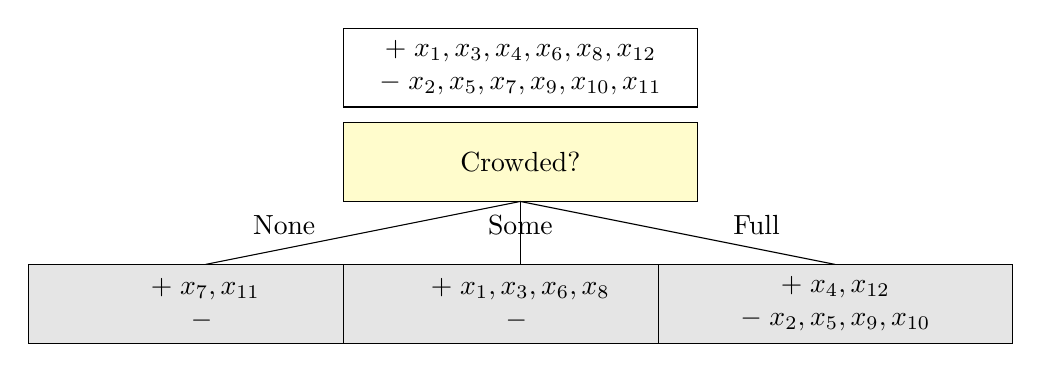
\begin{tikzpicture}[
        box/.style={draw, rectangle, minimum width=4.5cm, minimum height=1cm, align=center},
        yellowbox/.style={box, fill=yellow!20},
        graybox/.style={box, fill=gray!20},
        level 1/.style={sibling distance=6cm},
        level 2/.style={sibling distance=3cm},
        edge from parent/.style={draw, -}
      ]
        % Root node
        \node[box] {$+ \; x_1,x_3,x_4,x_6,x_8,x_{12}$ \\ $- \; x_2,x_5,x_7,x_9,x_{10},x_{11}$};
        \node[yellowbox] at (0,-1.2) {Crowded?};
        
        % Level 1 nodes and edges
        \node[graybox] at (-4,-3) {$+ \; x_7,x_{11}$ \\ $- \; $};
        \node[graybox] at (0,-3) {$+ \; x_1,x_3,x_6,x_8$ \\ $- \; $};
        \node[graybox] at (4,-3) {$+ \; x_4,x_{12}$ \\ $- \; x_2,x_5,x_9,x_{10}$};
        
        % Draw edges
        \draw (0,-1.7) -- (-4,-2.5);
        \draw (0,-1.7) -- (0,-2.5);
        \draw (0,-1.7) -- (4,-2.5);
        
        % Labels for edges
        \node at (-3,-2) {None};
        \node at (0,-2) {Some};
        \node at (3,-2) {Full};
      \end{tikzpicture}
      \caption{Visual of decision tree splitting according to how crowded it is. } 
      \label{fig:crowded_restaurants}
    \end{figure}
    
    In this case, we can define the multinomial distribution $X_{\mathrm{crowded}}$ representing the proportion of the data that is crowded in a specific level. That is, $X_{\mathrm{crowded}} \sim \mathrm{Multinomial}(\frac{2}{12}, \frac{4}{12}, \frac{6}{12} \big)$, with 
    \begin{equation}
      \mathbb{P}(X_{\mathrm{crowded}} = x) = \begin{cases} 2/12 & \text{ if } x = \text{ none} \\ 4/12 & \text{ if } x = \text{ some} \\ 6/12 & \text{ if } x = \text{ full} \end{cases}
    \end{equation}
    Therefore, we can now compute the conditional entropy of this new decision tree conditioned on how crowded the store is 
    \begin{align}
      H(Y \mid X_{\mathrm{crowded}}) & = \sum_x \mathbb{P}(X_{\mathrm{crowded}} = x) H(Y \mid X_{\mathrm{crowded}} = x) \\
      & = \frac{2}{12} H(\mathrm{Bern}(1)) + \frac{4}{12} H(\mathrm{Bern}(0)) + \frac{6}{12} H(\mathrm{Bern}(1/3)) = 0.459 \\
      I(Y; X_{\mathrm{crowded}}) & = 0.541
    \end{align}
    We would do this for all the features and greedily choose the feature that maximizes our information gain. 
  \end{example}

  \begin{example}[Ferrari F1 Race]
    The Ferrari F1 team hired you as a new analyst! You were given the following table of the past race history of the team. You were asked to use information gain to build a decision tree to predict race wins. First, you will need to figure out which feature to split first. 
    \begin{center}
      \begin{tabular}[c]{c|c|c||c}
      Rain & Good Strategy & Qualifying & Win Race \\ \hline
      1 & 0 & 0 & 0 \\
      1 & 0 & 0 & 0 \\
      1 & 0 & 1 & 0 \\
      0 & 0 & 1 & 1 \\
      0 & 0 & 0 & 0 \\
      0 & 1 & 1 & 1 \\
      1 & 0 & 1 & 0 \\
      0 & 1 & 0 & 1 \\
      0 & 0 & 1 & 1 \\
      0 & 0 & 1 & 1 \\
      \end{tabular}
    \end{center}

    Let $X \sim \mathrm{Bernoulli}(1/2)$ be the distribution of whether a car wins a race over the data. Then its entropy is 
    \begin{equation}
      H(X) = \mathbb{E}[-\log_2 p(x)] = \frac{1}{2} \big( -\log_2 \frac{1}{2} \big) + \frac{1}{2} \big( -\log_2 \frac{1}{2} \big) = 1
    \end{equation}

    Let $R \sim \mathrm{Bernoulli}(4/10), G \sim \mathrm{Bernoulli}(2/10), Q \sim \mathrm{Bernoulli}(6/10)$ be the distribution of the features rain, good strategy, and qualifying over the data, respectively. Then, the conditional entropy of $X$ conditioned on each of these random variables is 
    \begin{align*}
      H(X \mid R) & = \mathbb{P}(R = 1)\, H(X \mid R = 1) + \mathbb{P}(R = 0) \, H(X \mid R = 0) \\
      & = \frac{4}{10} \cdot - \big( 1 \cdot \log_2 1 + 0 \cdot \log_2 0 \big) + \frac{6}{10} \cdot - \big( \frac{1}{6} \cdot \log_2 \frac{1}{6} + \frac{5}{6} \cdot \log_2 \frac{5}{6} \big) \approx 0.390 \\
      H(X \mid G) & =  \mathbb{P}(G = 1)\, H(X \mid G = 1) + \mathbb{P}(G = 0) \, H(X \mid G = 0) \\
      & = \frac{2}{10} \cdot - \big( 1 \cdot \log_2 1 + 0 \cdot \log_2 0 \big) + \frac{8}{10} \cdot - \big( \frac{3}{8} \cdot \log_2 \frac{3}{8} + \frac{5}{8} \log_2 \frac{5}{8} \big) \approx 0.763\\
      H(X \mid Q ) & = \mathbb{P}(Q = 1)\, H(X \mid Q = 1) + \mathbb{P}(Q = 0) \, H(X \mid Q = 0) \\
      & = \frac{6}{10} \cdot - \big( \frac{4}{6} \cdot \log_2 \frac{4}{6} + \frac{2}{6} \cdot \log_2 \frac{2}{6} \big) + \frac{4}{10} \cdot - \big( \frac{1}{4} \log_2 \frac{1}{4} + \frac{3}{4} \log_2 \frac{3}{4} \big) \approx 0.875
    \end{align*}

    Therefore, the information gain are 
    \begin{align*}
        I(X; R) & = 1 - 0.390 = 0.610 \\
        I(X; G) & = 1 - 0.763 = 0.237 \\
        I(X; Q) & = 1 - 0.875 = 0.125 
    \end{align*}
    And so I would split on $R$, the rain, which gives the biggest information gain. 
  \end{example}

  Finally, we can use the Gini index of $X \sim \mathrm{Bernoulli}(p)$, defined 
  \begin{equation}
    G(X) = 2 p (1 - p)
  \end{equation}

  \begin{example}[Ferrari Example Continued]
    We do the same as the Ferrari example above but now with the Gini reduction. Let $X \sim \mathrm{Bernoulli}(1/2)$ be the distribution of whether a car wins a race over the data. Then its Gini index, which I will label with $\mathcal{G}$, is \[\mathcal{G} (X) = 2 \cdot \frac{1}{2} \cdot \frac{1}{2} = \frac{1}{2}\]
    Let $R \sim \mathrm{Bernoulli}(4/10), G \sim \mathrm{Bernoulli}(2/10), Q \sim \mathrm{Bernoulli}(6/10)$ be the distribution of the features rain, good strategy, and qualifying over the data, respectively. Then we compute the conditional expectation 
    \begin{align*}
        \mathbb{E}[\mathcal{G}(X \mid R)] & = \mathbb{P}(R = 1)\, \mathcal{G}(X \mid R = 1) + \mathbb{P}(R = 0) \, \mathcal{G}(X \mid R = 0) \\ 
        & = \frac{4}{10} \bigg[ 2 \cdot \frac{4}{4} \cdot \frac{0}{4} \bigg] + \frac{6}{10} \bigg[ 2 \cdot \frac{1}{6} \cdot \frac{5}{6} \bigg] \approx 0.167 \\
        \mathbb{E}[\mathcal{G}(X \mid G)] & = \mathbb{P}(G = 1)\, \mathcal{G}(X \mid G = 1) + \mathbb{P}(G = 0) \, \mathcal{G}(X \mid G = 0) \\ 
        & = \frac{2}{10} \bigg[ 2 \cdot \frac{2}{2} \cdot \frac{0}{2} \bigg] + \frac{8}{10} \bigg[ 2 \cdot \frac{3}{8} \cdot \frac{5}{8} \bigg] \approx 0.375 \\
        \mathbb{E}[\mathcal{G}(X \mid Q)] & = \mathbb{P}(Q = 1)\, \mathcal{G}(X \mid Q = 1) + \mathbb{P}(Q = 0) \, \mathcal{G}(X \mid Q = 0) \\ 
        & = \frac{6}{10} \bigg[ 2 \cdot \frac{4}{6} \cdot \frac{2}{6} \bigg] + \frac{4}{10} \bigg[ 2 \cdot \frac{1}{4} \cdot \frac{3}{4} \bigg] \approx 0.417
    \end{align*}
    Therefore, the Gini reduction, which I'll denote as $I_{\mathcal{G}}$, is 
    \begin{align*}
        I_{\mathcal{G}} (X ; R) & = 0.5 - 0.167 = 0.333 \\
        I_{\mathcal{G}} (X ; G) & = 0.5 - 0.375 = 0.125 \\
        I_{\mathcal{G}} (X ; Q) & = 0.5 - 0.417 = 0.083
    \end{align*}
    Since branching across the feature $R$, the rain, gives the biggest Gini reduction, we want to split on the rain feature first. 
  \end{example}


\subsection{Surrogate Loss}

\subsection{CART} 

\subsection{ID3} 

\subsection{c4.5} 


\section{Regularization} 

  Given a dataset with $D$ binary features, let $g(H, D)$ be the number of binary trees with depth at most $H$ (including root node), with the restriction that the trees may not split on some variable multiple times within a path to a leaf node. Then, $g$ can be defined recursively. 
  \begin{enumerate}
      \item First, if $H = 1$, then $g(H, D) = 1$ always since we are just creating the trivial binary tree of one node. 
      \item If $D = 0$, then there are no features to split on and therefore we just have the single node $g(H, D) = 1$. 
      \item If $H > 1$ and $D > 0$, then say that we start with a node. We can either make this a leaf node by not performing any splitting at all, or split on one of the $D$ variables. Then for each of the 2 nodes created on the split, we are now working with $D-1$ features and a maximum height of $H-1$ for each of the subtrees generated from the 2 nodes. 
  \end{enumerate}
  All this can be expressed as 
  \[g(H, D) = \begin{cases} 1 + D \, \big[ g(H - 1, D - 1) \big]^2 & \text{ if } H > 1, D > 0 \\ 1 & \text{ if } H = 1 \text{ or } D = 0 \end{cases} \]
  which is extremely large (in fact, NP hard). Therefore, some tricks like regularization must be implemented to limit our search space. 

  By defining the complexity of our decision tree $\Omega(h)$ as the number of nodes within the tree, we can modify our objective function to 
  \[L(h; \mathcal{D}) = \frac{1}{N} \sum_{i=1}^N 1_{\{y^{(i)} \neq h(x^{(i)})\}} + \lambda \Omega(h)\]
  We can impose this constraint directly on the training algorithm, or we can calculate the regularized loss after the tree has been constructed, which is a method called \textbf{tree pruning}. 

  Given a large enough $\lambda$, we can in fact greatly reduce our search space by not considering any trees further than a certain point. 

  \begin{theorem}
  We describe a tree as a set of leaves, where leaf $k$ is a tuple containing the logical preposition satisfied by the path to leaf $k$, denoted $p_k $, and the class label predicted by the leaf, denoted $\hat{y}_k$. For a dataset with $d$ binary features, $p_k: \{0, 1\}^d \to \{0, 1\}$ is a function that returns $1$ if a sample $x_i$ satisfies the preposition, and $0$ otherwise. That is, leaf $k$ is $(p_k, \hat{y}_k),$ and a tree $f$ with $K$ leaves is described as a set $f = \{(p_1, \hat{y}_1), \hdots, (p_K, \hat{y}_K)\}$. Assume that the label predicted by $\hat{y}_k$ is always the label for the majority of samples satisfying $p_k$. Finally, let $m_k = \sum_{i=1}^n p_k(x_i)$ denote the number of training samples ``captured'' by leaf $k$.

  Given a (potentially optimal) tree 

    \[f = \{(p_1, \hat{y}_1), \hdots, (p_{\kappa}, \hat{y}_{\kappa}), \hdots, (p_K, \hat{y}_K)\}, \]

  the tree $f' = \{(p_1, \hat{y}_1), \hdots, (p_{\kappa_1}, \hat{y}_{\kappa_1}), (p_{\kappa_2}, \hat{y}_{\kappa_2}), \hdots, (p_K, \hat{y}_K)\}$ produced by splitting leaf $(p_{\kappa}, \hat{y}_{\kappa})$ into two leaves $(p_{\kappa_1}, \hat{y}_{\kappa_1})$ and $(p_{\kappa_2}, \hat{y}_{\kappa_2})$ and any tree produced by further splitting $(p_{\kappa_1}, \hat{y}_{\kappa_1})$ or $(p_{\kappa_2}, \hat{y}_{\kappa_2})$ cannot  be optimal if $m_{\kappa} < 2n\lambda$.
  \end{theorem}
  \begin{proof}
  Let $c$ be the number of misclassifications in leaf $(p_{\kappa}, \hat{y}_{\kappa})$. Since a leaf classifies according to the majority of $m_{\kappa}$, we must have 

    \[c \leq \frac{m_\kappa}{2} < n \lambda\]

  By splitting leaf $(p_\kappa, \hat{y}_\kappa)$ into leaves $(p_{\kappa_1}, \hat{y}_{\kappa_1})$ and $(p_{\kappa_2}, \hat{y}_{\kappa_2})$, assume that we have reduced the number of misclassifications by $b \leq c$. Then, we have 

    \[\ell(f^\prime, \mathbf{X}, \mathbf{y}) = \ell(f, \mathbf{X}, \mathbf{y}) - \frac{b}{n}\]

  However, we have increased the number of leaves by $1$, and so 

    \[\lambda s(f^\prime) = \lambda s(f) + \lambda\]

  Combining the last two equations, we have obtained 

    \[R (f^\prime, \mathbf{X}, \mathbf{y}) = R(f, \mathbf{X}, \mathbf{y}) + \lambda - \frac{b}{n}\]

  However, we know that 

  \begin{align*}
    b \leq c & \implies \frac{b}{n} \leq \frac{c}{n} < \frac{n \lambda}{n} = \lambda \\
    & \implies - \frac{b}{n} > - \lambda \\
    & \implies \lambda - \frac{b}{n} > \lambda - \lambda = 0
  \end{align*}

  and so $R (f^\prime, \mathbf{X}, \mathbf{y}) > R(f, \mathbf{X}, \mathbf{y})$. This means that $f^\prime$ cannot be optimal according to our regularized objective. We have also proved that further splitting $(p_{\kappa_1}, \hat{y}_{\kappa_1})$ or $(p_{\kappa_2}, \hat{y}_{\kappa_2})$ cannot  be optimal since we can just set $f = f^\prime$, and apply the same argument. 
  \end{proof}

\subsection{Pruning} 

\subsection{Splitting} 

\section{Improved Optimization} 

\subsection{GODST} 

\section{Soft Decision Trees} 

\subsection{Soft Splitting}

\subsection{Neural Decision Trees}


\bibliography{./bibfile}
\bibliographystyle{alpha}

\end{document}
